\documentclass[12pt, a4paper]{jreport}

\usepackage[driver=dvipdfm]{geometry}
\usepackage[dvipdfmx]{graphicx, color}
\usepackage{here}
\usepackage{plext}
\usepackage{times, mathptmx}
\usepackage{longtable}
\usepackage{colortbl}
\usepackage{tabularx}
\usepackage{enumerate}
\usepackage{comment}
\usepackage{url}
\usepackage{lscape}
\usepackage{multirow}
\usepackage{amsmath}
\usepackage{mathtools}
\usepackage{bm}
%\usepackage{otf}

\setlength{\voffset}{0.5truecm}
\setlength{\headsep}{2truecm}
\setlength{\oddsidemargin}{7.0truemm}
\setlength{\evensidemargin}{-5.5truemm}
\setlength{\topmargin}{-1truecm}
\setlength{\footskip}{25truemm}
\setlength{\textwidth}{15truecm}
\setlength{\textheight}{22truecm}
\makeatletter
\makeatother

\begin{document}
    \thispagestyle{empty}
    \begin{center}

        \vspace{20mm}
        {\Large\noindent 2023年度 卒業論文}\\
        \vspace{40mm}
        {\huge\noindent\textbf{プログラムコードの複雑さの防止効果が高いシステム開発上の要素の検討}}\\
        \medskip
%{\huge\noindent\textbf{論文タイトル(2行目)}}\\
        \vspace{\baselineskip}
        {\LARGE\noindent\textbf{Proposition of viewpoints}}\\
        \medskip
        {\LARGE\noindent\textbf{on prevention of program code complexity }}\\
        \medskip
        {\LARGE\noindent\textbf{in system development}}\\
        \vspace{40mm}

        {\Large\noindent
        2024年2月9日\\
        \vspace{\baselineskip}
        指導教員 山川 広人   \\
        \vspace{\baselineskip}
        公立千歳科学技術大学 理工学部\\
        情報システム工学科 山川研究室\\
        \vspace{\baselineskip}
        B2201400 須藤 真由 \\
        }
        \vspace{40mm}

    \end{center}
    \pagenumbering{roman}
    \tableofcontents
    \chapter{序論}
    \pagenumbering{arabic}

    \section{背景}
    複雑なプログラムコードがシステム開発上やプログラミング教育の上で障壁となることがある。プログラムコードの複雑さに対する取り組みや議論は盛んであり、システム開発上の観点として、株式会社サイバーエージェント\cite{CyberZ}では、新卒採用されたエンジニア向けにプログラムコードの品質に関する講義を行っている。プログラムコードの品質を上げることでプログラムコードの可読性が向上し、速い開発スピードを維持できると説明している。開発スピードの速さは市場での競争力に影響を与えることにも言及している。また、松田\cite{kireina}はきれいなプログラムを継続的に記述していくために気を付けるべきことについてまとめており、1つのメソッドが長くなることで発生する複雑さや、適切な命名を行うことで読みやすくなることについて述べている。プログラミング教育上の観点として、平嶋ら\cite{haikei}は高等教育機関におけるプログラミング講義に苦手意識を持つ学習者に着目し,プログラミング学習者の認知負荷を減少させ、アルゴリズムの組み立て等の適切な部分に集中できるようにするために、カードを並べ替える方式の学習方法を提案した。このように様々な観点でのプログラムコードに関わる複雑さが検討され、またそれらは学習やシステム開発をする上で問題となり得るため、システムの継続的な発展やより効果的なプログラミング教育の実現などの面でも解決すべき課題と捉えることができる。
    \\ プログラムコードの複雑さに関わる研究は、システム開発上の観点、教育上の観点の両面を兼ね備える、実システム開発を題材としたPBL(Project Based Learning)学習に対しても有用であろう。PBL学習には企業や地域のステークホルダーと連携し、数世代に亘ってプロジェクトを引継ぐことで成果物の発展や価値提供を行い続けるものがある。特に、プログラムコードが関わる複雑さの中で、プログラムコードが要件や設計を適切に反映しているか、プログラムコードから実現する要件や実装する設計が読み解きやすいかの観点で内部構造が複雑化している情報システムなどを例にすると、学生がプログラムコードから要件や仕様を理解することも難しくなり、ひいては新たな価値へ向けた発展的開発も実現しずらいものとなる。この観点でのプログラムコードの複雑さに関わる原因やそれを防止する方法について明らかにすることは、PBL 学習を効果的に行うためにも重要となる。
\section{目的}
本研究は、プログラムコードから実現する要件や実装する設計が読み解きやすいかの観点でのプログラムコードの複雑さを防止する方法を明らかにすることを目的とする。これにむけて、システム開発に携わる開発者役となる学生が、情報システムによるサービス化をしたい対象(ドメイン)へのエキスパートと協同で進めるシステム開発PBL によるシステムを題材とする。プログラムコードの複雑さが招かれる3つの要素を提案し、これらの要素をシステム開発上のモデリングやテストに関わる手法の工夫で複雑さを改善できるかを検討する。検討した結果をもとに、どのような方策を新たに取り入れることでプログラムコードの複雑さを防止できるか考察する。
\section{構成}
本論文は全6章で構成している。第2章で関連している研究と本研究の位置づけについて述べる。第3,4章でリサーチクエスチョン1について、複雑なプログラムコードの分析結果と改善案について述べる。第5章でリサーチクエスチョン2について、評価方法の検討と結果、結果を踏まえた考察について述べる。第6章では第3,4,5章を踏まえ本研究の結論を述べる。
\chapter{先行研究と本研究の位置づけ}
\section{先行研究}
\subsection{認知負荷に着目したプログラミング学習方法を提案している事例}
1.1で述べたとおり、平嶋ら\cite{haikei}は高等教育機関におけるプログラミング講義に苦手意識を持つ学習者に着目し,プログラミング学習者の認知負荷を減少させ、アルゴリズムの組み立て等の適切な部分に集中できるようにするために、カードを並べ替える方式の学習方法を提案している。この研究ではこれはプログラムコードに関する複雑さの中でも、文法的な複雑さの解消に向けた提案である。
\subsection{ドメイン駆動設計を用いた開発の効率化の事例}

\subsection{きれいなプログラムコードについてまとめている事例}

\subsection{変更容易性に着目した授業設計を提案している事例}

\section{本研究の位置づけ}
様々な方向の複雑さに研究は進んでいるが、本研究はコードから要求や仕様を読み取ることの複雑さ、また将来的なPBLへの応用を考える上で、連携しているステークホルダーに要求や仕様を共有することに対する複雑さを課題と捉え検証していく。
\chapter{複雑さの原因の分析と改善案の提案}
\section{研究の対象とするシステム}
プログラムコードの複雑さを招いている現状を分析し、複雑さの原因を明らかにする。複雑化したプログラムコードとして公立千歳科学技術大学で開発が進められてきた既存のシステムである「話しことばチェッカー」のプログラムコードを用いる。このシステムは文章を入力し検出ボタンを押すと文章内から話しことばを検出し、修正例と共に検出結果を示す文章校正システムである。下の図3.1にこのシステムの処理の流れを示す。
\begin{figure}[H]
\centering
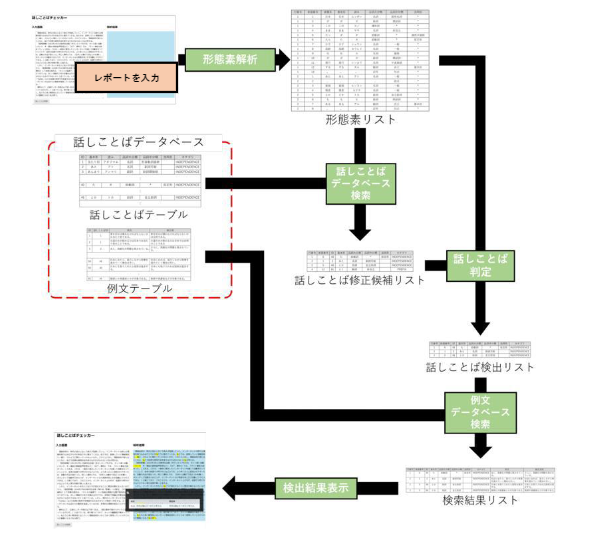
\includegraphics[width=1\linewidth]{image/cqcNagare.png}
\caption{話しことばチェッカーのシステムの処理の流れ(開発プロジェクトの責任者である教員の論文\cite{Yamashita}から引用)}
\label{fig:enter-label}
\end{figure}
このシステムは2018年度から開発が開始され、現時点で5年が経過している。開発は実システム開発を題材としたPBLの中で行われ、開発プロジェクトの責任者である話しことばチェッカーのエキスパート教員(3.3.1で後述するドメインエキスパート)や、技術やスケジュール等をメンタリングするメンター教員は変わらないものの、求められる要件の定義や設計、それを実装として反映するプログラミングは年度ごとに異なるPBL参加学生が、前年度までの成果を引き継ぎながら開発を任される形で行ってきた。図3.1に、開発体制を示す。
\begin{figure}[H]
\centering
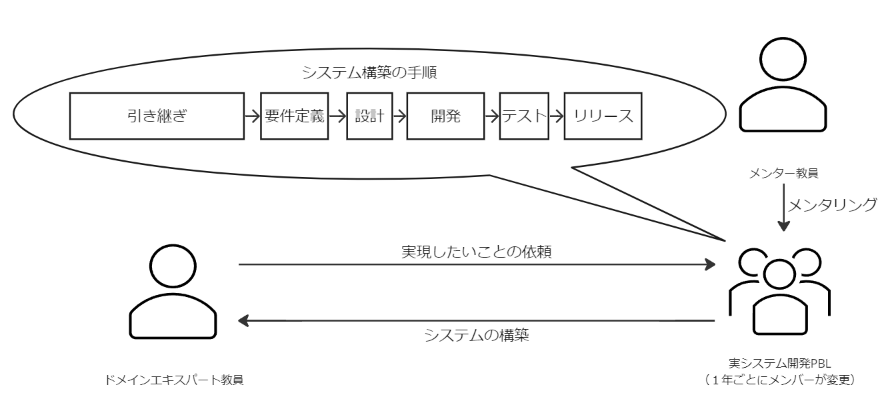
\includegraphics[width=0.75\linewidth]{image/taisyou1.1.png}
\caption{研究対象のシステムの開発体制}
\label{fig:enter-label}
\end{figure}
開発体制の中、ドメインエキスパートが実現したいこと(話し言葉の検出・修正例の提示、およびそれらの年度ごとの改良)のシステム化に必要な要件定義や設計・実装はPBLの学生たちに任されている形であった。システムの開発言語はJavaで行われており、その規模は49クラス、2954行に上る。また、学習者はPBL の中で経験の浅いシステム開発者であることから、引き継ぎやその後の発展的な開発への準備も難しく、システム開発の中で作り上げた要件定義や設計を参照できるドキュメント等の整備や更新も十分なものとは言えない状況である。
\\ こうした中で、前年度の成果を新たな学生が引き継ぐ際、プログラムのコードを手がかりに、要件や設計を読み取り理解し進めていく必要がある。しかしながらこれに携わる学生からはシステムが見かけ上正しく動作しているように見えるが、それを実現するプログラミングコードの間のつながりや役割が難解であり、想定されている要件や設計とプログラムコードの対応の想起や認知が難しいことが悩みの声として上がっていた。当然、この解決にはドキュメントの整備不足の影響や整備方法の課題検討の余地はあるが、本研究ではそれとは別の課題として、プログラムコードから要件や設計を読み取ることが難しいという観点で、難解な複雑さを持つプログラムコードが生成されている問題を重要なものとして捉える。本卒業論文では以降も、プログラムコードの複雑さを、プログラムコードから要件や設計を読み取り理解することの難しさとして捉え議論していく。
\section{複雑さの原因の分析}
本研究は3.1で述べた状況からもシステムが5年間の開発の中で複雑化を引き起こしていると考え、プログラムコードを読み複雑さの原因となる問題点を以下の3つの観点から検討することにした。
\begin{enumerate}
\item サービス化をしたい対象について役割と処理範囲が明確ではないコードであること
\item サービス化をしたい対象について開発者独自の解釈しか反映されていないコードであること
\item サービス化をしたい対象について想定される処理結果と実際の結果を確認できないコードであること
\end{enumerate}
1について、以下に示した図3.1のプログラムコードのように1つのメソッドに多くの役割が含まれていること、話しことばの検出にまつわるメソッドがまとめて1つのクラスに書かれており、検出についての詳細な処理がどこに書かれているか探しにくい状態になっていた。
\begin{figure}[H]
\centering 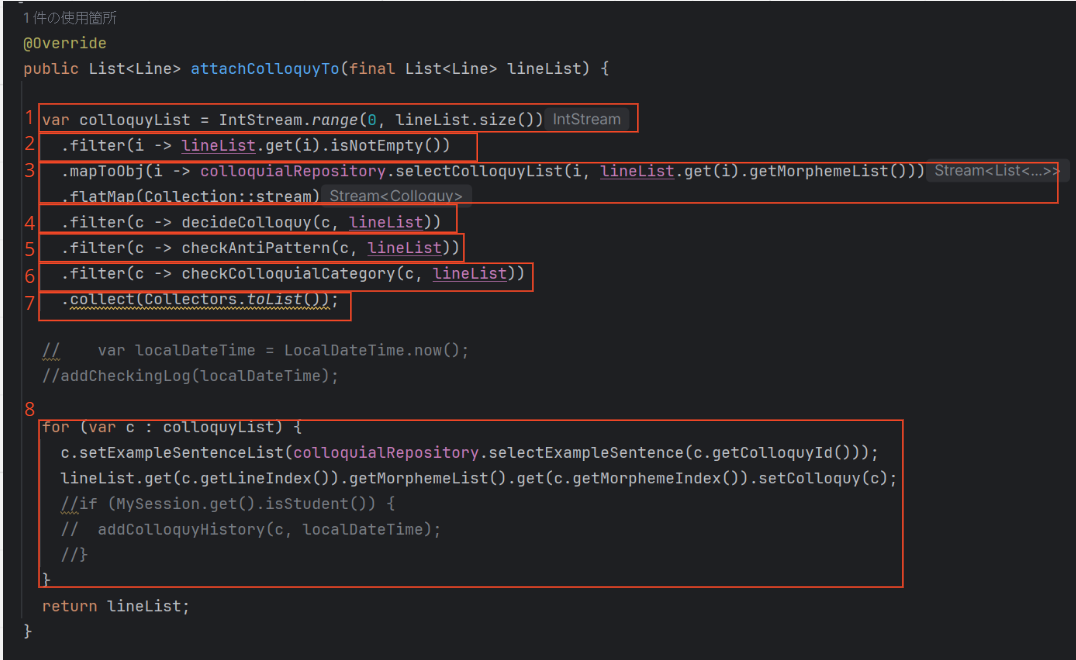
\includegraphics[width=1\linewidth]{image/genin1.1.png}
\caption{どのような役割がどこに書かれているのか分からないコードの例}
\label{fig:enter-label}
\end{figure}
2について、話しことばの検出の過程には形態素解析を行った後に形態素の前後関係を用いるものがあり、それらをカテゴリで分類し判断している。その中で、下に示す図3.2のクラス構造の赤丸で示したようにいくつか前の形態素を用いるものを"C2"や"Prefix"、「1つ」、「2つ」、「3つ」をドイツ語で"Eins"、"Zwei"、"Drei"等のように開発者独自の命名でプログラムコード上に示している。こういった命名の他、処理の内容や順番に開発者独自の考えが反映されていた。
\begin{figure}[H]
\centering
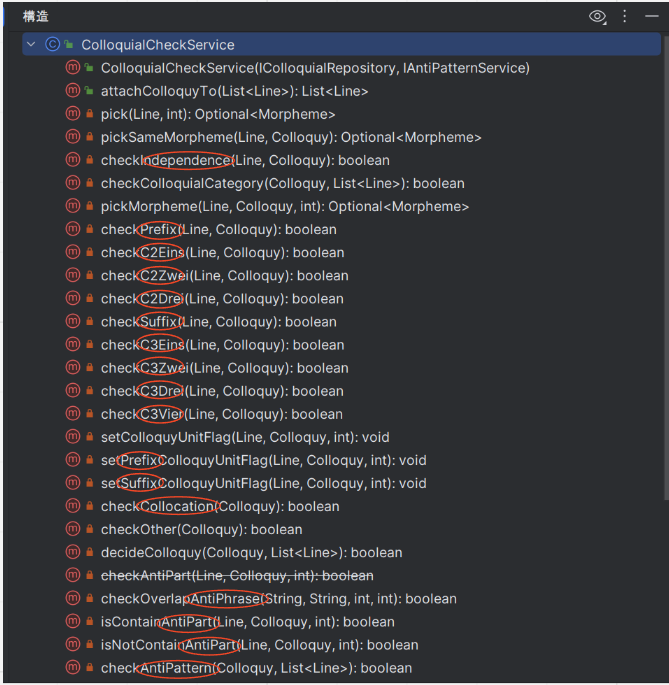
\includegraphics[width=1\linewidth]{image/genin2.1.png}
\caption{開発者の独自の解釈を反映させたコードの例}
\label{fig:enter-label}
\end{figure}
3について、このシステムがどのような操作でどのような結果を示すものなのか、どのような実装がされていればステークホルダーの要求を満たしているのか、確かめる手段が用意されていなかった。したがってこれまでのPBLではシステムを実際に動かし、結果に相違がないか目視で確認する方法でリリース前のテストを行っていた。
\section{複雑さの防止方法の提案}
プログラムコードの複雑さの原因に基づき、改善する方法として適切なモデリングとテストコードの整備が有効であると仮定して、リファクタリングを行いプログラムコードを改善する。
\subsection{モデリング}
モデリングの見直しを行う。清田\cite{Domein}はドメイン駆動設計によりシステム開発を行う中で、モデル作成時のポイントとして「ビジネスロジックの詳細仕様書として業務資料そのものを利用すること」を挙げている。ドメイン駆動設計はシステムによって解決したい問題領域をドメインと呼び、それをシステム構造に反映させるシステム設計手法である。また、ドメインについて深く理解している、実業務の有識者をドメインエキスパートと呼び、ドメインエキスパートの協力を得ながらシステム設計を進める。業務で利用される判断条件や計算式のことであるビジネスロジックを基にドメインモデルを作成するために、清田は実際の業務で利用されているドキュメントからビジネスロジックを抽出した。また、ソースコードのクラス名、メソッド名、変数名についてもそれらの業務マニュアルに合わせることによって、ユーザーでも理解しやすいプログラムソースを追及している。このように、サービス化したい対象について、ドメインエキスパートの知識が反映された文章をもとにビジネスロジックを抽出し、ソースコードに反映する手法を取り入れたモデリングを行うことは、ビジネスロジックの実現に向けてどのプログラムコードがどのような役割を果たさなくてはならないかを文章中の表現(例えば主語や名詞をクラス名、述語をメソッド名)として対応づけしやすくなる点で、3.2 に述べた複雑さの原因1に寄与する可能性が考えられる。さらにこれが実現されていれば、ドメインエキスパートの知識が反映された文章の流れと、ソースコード上での処理の流れの対応を開発者だけではなくドメインエキスパートとも確認しやすくなる点で、複雑さの原因2に寄与する可能性が考えられる。
\\ このモデリング手法を本研究の事例の話し言葉チェッカーに応用することを考えると、本研究では話しことばチェッカーの共同研究者でありドメインに深く通じている山下の論文\cite{Yamashita}を詳細仕様書として利用する。山下の論文を基にビジネスロジックを適切に分割し、クラス名やドメインモデルに使用するチーム全体で意図を共有する言葉であるユビキタス言語も山下の論文に合わせる。このようにモデリングを行うことで、「どのような役割がどこに書かれているのか分からないコード」という点と「開発者の独自の解釈を反映させたコード」という点の改善に有効であると想定している。
\subsection{テストコードの作成}
単体テストを作成する。Vladimir Khorikov\cite{Tantai}はシステム開発プロジェクトの成長を持続可能なものにするために単体テストが有効であると述べている。テストがあることで、プログラムコードに変更を加えた際に、意図したように機能しなくなったことやバグの発生を検出することができる。テストを用いることで、既存の機能が正しく動作することを確信できるようになるため、新しい機能の追加や新たな要求を満たすリファクタリングといったプロジェクトを成長させる活動に取り組みやすくなるのである。また、プログラムコードにどのような観察可能な振る舞いがあるのかを理解することにもテストコードは有用である。観察可能な振る舞いとは、そのプログラムコードを呼び出すプログラムコードや外部クライアントやアプリケーション等において、呼び出す際に行われた操作やその際の状態のことである。つまり、どこでどのような操作が行われるのか、どこがどのような状態になっているのかを示すものである。このように、サービス化したい対象について、ドメインエキスパートや開発者が想定する処理の一覧とその結果(振る舞い)をそれぞれ観察可能にすることは、開発者が想定される処理結果と実際の結果を確認がしやすくなる点で、複雑さの原因3に寄与する可能性がある。さらにこれが実現されていれば、ドメインエキスパートが想定するシステムのふるまいと開発者が想定するシステムの振る舞いを照らし合わせやすくなる点で、複雑さの原因2に寄与する可能性がある。
\\ このテスト手法を本研究の事例の話し言葉チェッカーに応用することを考えると、本研究ではリファクタリング前後で振る舞いが変わらないようにするため、またシステム内の操作や状態を把握することでこのシステムが正しく動作していると判断する方法を用意するために、観察可能な振る舞いの考えを基に、プレゼンテーション層とドメイン層へテストコードを取り入れる。(図3.4)テストコードを作成することで、「どのような操作でどのような結果を示すのか分からないコード」という点の改善に有効であると想定している。
\begin{figure}[H]
\centering
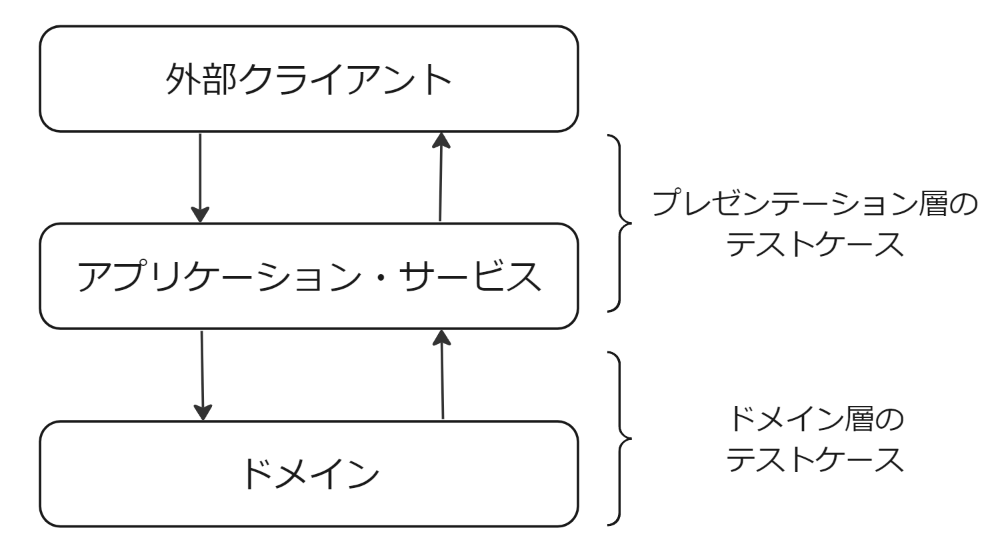
\includegraphics[width=1\linewidth]{image/layerTest.png}
\caption{テストコードを取り入れる}
\label{fig:enter-label}
\end{figure}
\chapter{リファクタリングによるコードの改善}
\section{改善方法}
3.3で提案した複雑さの防止方法について、実際のシステム開発の現場でドメイン駆動設計やテスト駆動開発に取り組むエンジニアの助言を得ながら、リファクタリングを進める。
\section{改善結果}
リファクタリングを経て、以下のように複雑さの原因を含んだプログラムコードを複雑さが解消されたプログラムコードに改善できた。
\begin{enumerate}
\item どのような役割がどこに書かれているのか分からないコードを、責務を分けたコードに改善
\item 開発者の独自の解釈を反映させたコードを、共有されたメンタルモデルを反映したコードに改善
\item どのような操作でどのような結果を示すのか分からないコードを、観察可能な振る舞いが確認できるコードに改善
\end{enumerate}
 山下の論文語を基にビジネスロジックを抽出し、ユビキタス言語やドメインモデルに使用したことで、下に示す図4.2のようなモデルへ変更された。1についてはユビキタス言語の一つ一つが責務を持つ構造のコードに改善した。2については日本語の単位をモデリングに取り入れたことで、問題の解決方法の解釈のことであるメンタルモデルをプログラムコードに反映した。それにより、命名や構造に開発者の独自の解釈を用いていないプログラムコードへと改善した。
\begin{figure}[H]
\centering
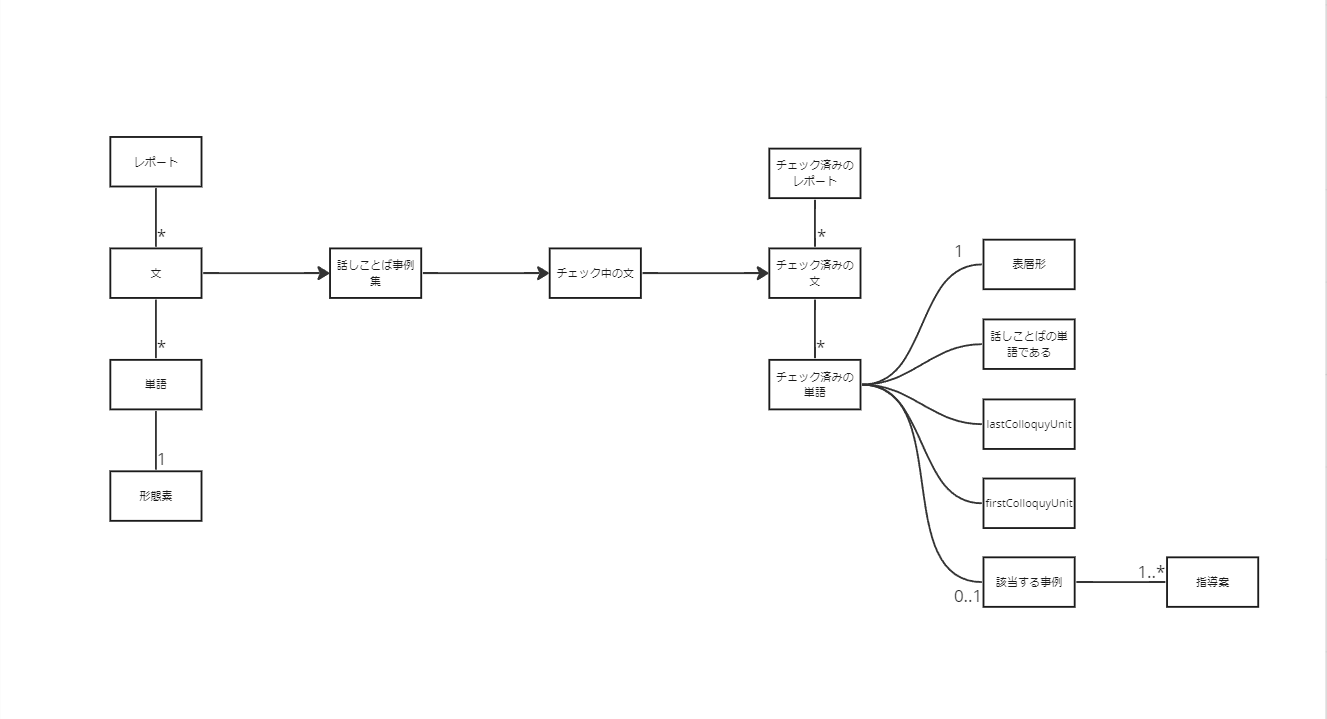
\includegraphics[width=1\linewidth]{image/kaizen2.png}
\caption{プログラムコードに反映したメンタルモデルの一部}
\label{fig:enter-label}
\end{figure}
元のプログラムコードは下に示す図4.1の赤い矢印より左のようなアーキテクチャであり、Service層に責務が集中していた。モデリングを行ったことにより赤い矢印より右のようなアーキテクチャへと変化した。1についてはDomain層に計算・加工・判断など話しことば検出に必要な責務を分離し、どこにどの責務があるのか、明確になった。2については各層に含まれるクラスを辿ることでメンタルモデルが反映されていることを確認し共有できるようになった。
\begin{figure}[H]
\centering
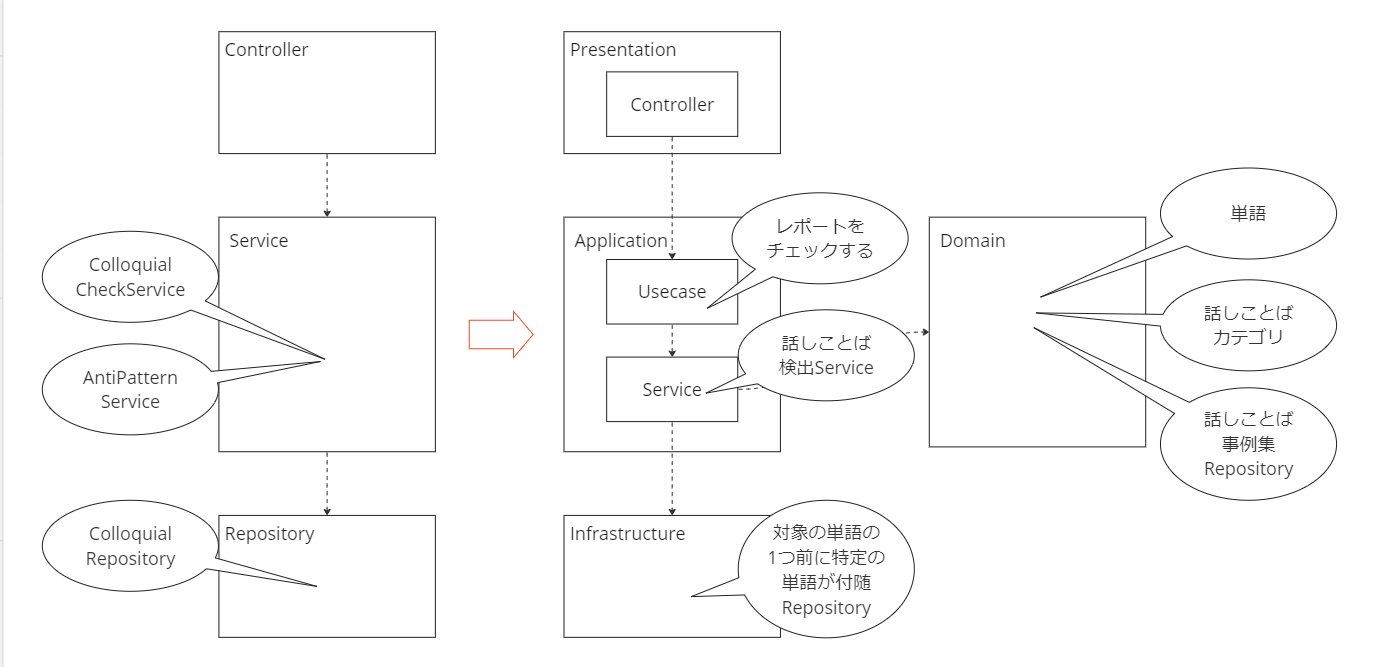
\includegraphics[width=1\linewidth]{image/kaizen1.png}
\caption{リファクタリングによるアーキテクチャの変化}
\label{fig:enter-label}
\end{figure}
3について、プログラムコードにテストコードを追加したことで、このシステムではどのような操作と結果が期待されているのか確認できるようになった。下の図4.3に示すようにテストケースの命名、入力と期待する出力にこういった観察可能な振る舞いを確認することができるようなプログラムコードに改善した。
\begin{figure}[H]
\centering
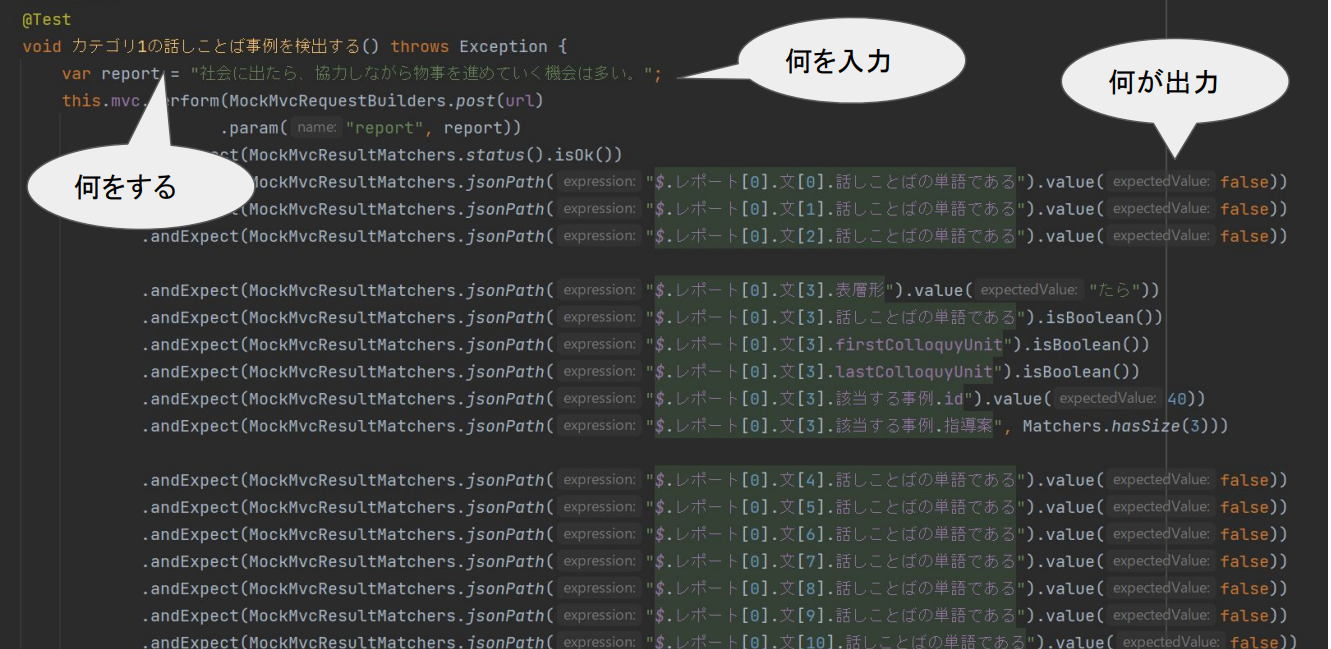
\includegraphics[width=1\linewidth]{image/kaizen3.png}
\caption{テストコードの例}
\label{fig:enter-label}
\end{figure}
下に示す図4.4と図4.5は作成したテストクラスの構造である。2,3について、メンタルモデルにどのような観察可能な振る舞いがあるか確認できるようになった。また、これを用いてそれらの振る舞いが正しく動いているか確認できるようになった。
\begin{figure}[H]
\centering
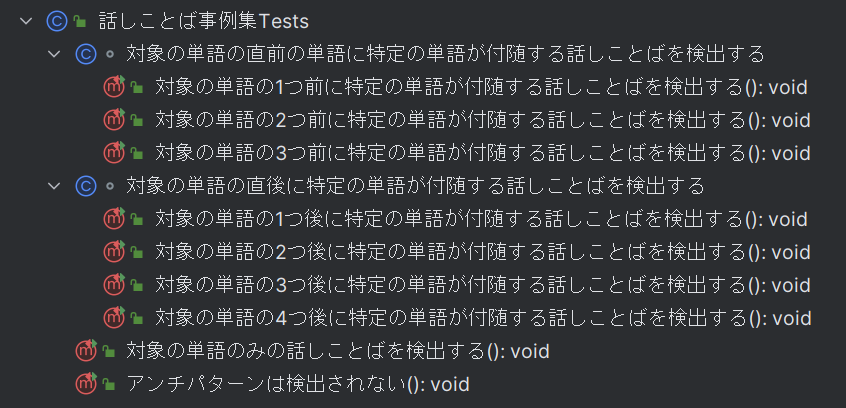
\includegraphics[width=1\linewidth]{image/presenTest.png}
\caption{プレゼンテーション層のテストクラス}
\label{fig:enter-label}
\end{figure}
\begin{figure}[H]
\centering
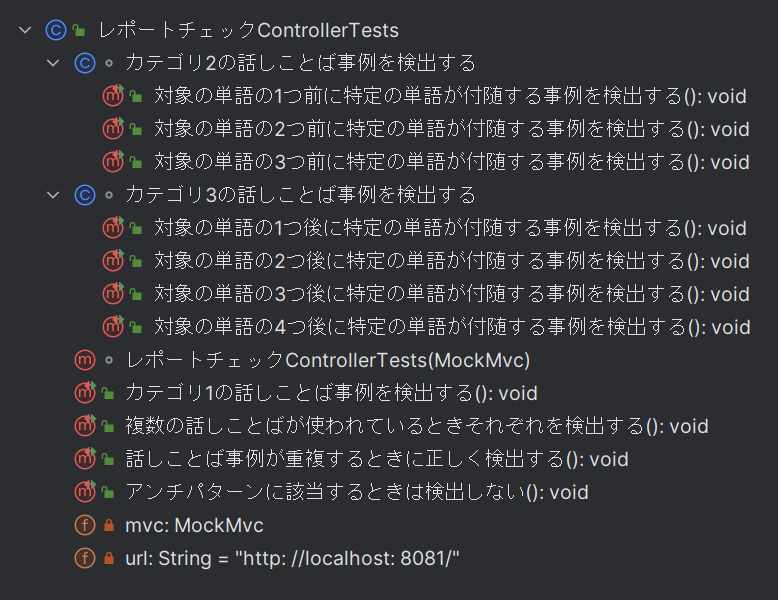
\includegraphics[width=1\linewidth]{image/domainTest.png}
\caption{ドメイン層のテストクラス}
\label{fig:enter-label}
\end{figure}
\chapter{評価方法の検討}
\section{評価方法}
\subsection{責務を分けたコード}
責務を分けたコードとなっているか、凝集度を用いた定量評価を行う。凝集度とはクラス内のデータとロジックの関係性の強さを表す指標であり、クラス内に責務がどの程度集中しているか示すことができるものである。
\\ 凝集度を計測できるツールとしてYegor Bugayenkoが公開しているjPeekの5つの指標で計測する。5つの指標は以下の通りである。
\\
\begin{gather}
\text{CAMC : }
\frac{a}{kl}
\end{gather}
\begin{gather*}
a\text{ メソッド内の型の数}
\\k\text{ メソッドの数}
\\l\text{ 型の数}
\end{gather*}
\\
\begin{equation}
LCOM5:
\frac{a-kl}{l-kl}
\end{equation}
\begin{gather*}
a\text{ メソッド内のattributesの数}
\\k\text{ メソッドの数}
l\\l\text{ attributesの数}
\end{gather*}
\\
\begin{equation}
MMAC:
\frac{\sum^{i=l}_{i=1}{{x}_{i}{({x}_{i}-1})}}{lk(k-1)}
\end{equation}
\begin{gather*}
l\text{ 型の数}
\\k\text{ メソッドの数}
\\{x}_{i}\text{ 戻り値が}i\text{のメソッドの数}
\end{gather*}
\\
\begin{equation}
NHD:
1-\frac{2}{lk(k-1)}\sum^{l}_{j=1}{x}_{i}{(k-{x}_{i})}
\end{equation}
\begin{gather*}
l\text{ 型の数}
\\k\text{ メソッドの数}
\\{x}_{i}\text{ }i\text{の型を含むメソッドの数}
\end{gather*}
\\
\begin{equation}
SCOM:
\frac{2}{m(m-1)}\sum^{m-1}_{i=1}\sum^{m}_{j=i+1}\frac{|{I}_{i}\cap{I}_{j}|}{min(|{I}_{i}|,|{I}_{j}|)}*\frac{|{I}_{i}\cup{I}_{j}|}{l}
\end{equation}
\begin{gather*}
m\text{ メソッドの数}
\\|{I}_{i}|\text{ }i\text{のattributesの濃度}
\\|{I}_{j}|\text{ }i\text{のattributesの濃度}
\\|{I}_{i}\cap{I}_{j}|\text{ }(i\text{のattributes}\cap j\text{のattributes)の濃度}
\\|{I}_{i}\cup{I}_{j}|\text{ }(i\text{のattributes}\cup j\text{のattributes)の濃度}
\\l\text{ attributesの数}
\end{gather*}
\\ これらの指標はスコアが高いほど凝集度が低く、責務が分けられていると一般的に言われている。これを用いてリファクタリング前後の凝集度を算出し、結果の比較を行う。
\subsection{共有されたメンタルモデルを反映させたコード}
リファクタリング前後のプログラムコードを文書化し、それを用いてドメインエキスパートにインタビューを行うことで、共有されたメンタルモデルが反映されたコードとなっているか定性評価を行う。
\\ 文書化にあたり、IDEであるintelliJでVanStudioが公開しているSequence Diagramというシーケンス図を生成するプラグインを利用する。生成したシーケンス図の一部を以下の図5.1に示す。これを用いて、メッセージを受け取るライフラインとメッセージの内容を助詞の「で」を用いて繋げ、処理が行われる順番通りに番号を振ることで文書化する。この文書を用いてメンタルモデルが合っているかどうか、メンタルモデルが合っている部分はコードに直接メンタルモデルを表現できているかについて、ドメインエキスパートである山下にインタビューを行う。
\begin{figure}[H]
\centering
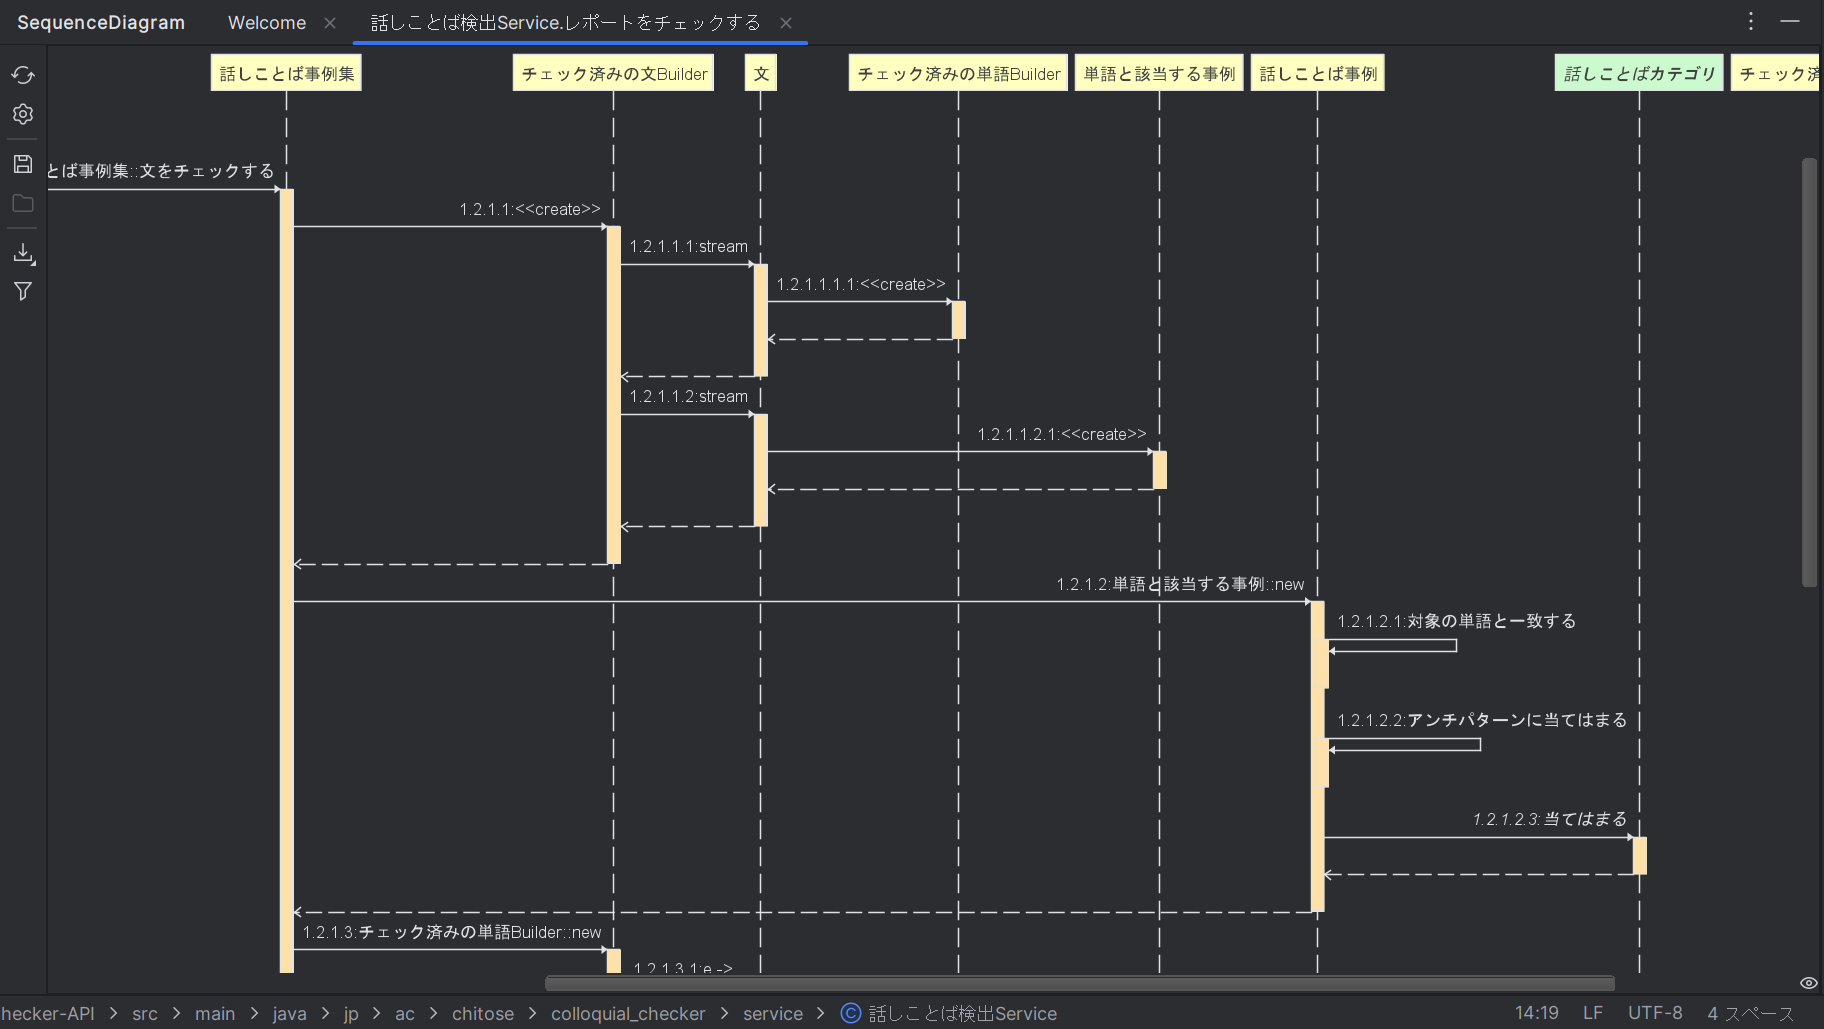
\includegraphics[width=1\linewidth]{image/sequence.png}
\caption{生成したシーケンス図の一部}
\label{fig:enter-label}
\end{figure}
\subsection{観察可能な振る舞いを確認できるコード}
テストコードを文書化し、それを用いてドメインエキスパートにインタビューを行うことで観察可能な振る舞いを確認できるコードとなっているか定性評価を行う。また、実際にテストコードを実行し、リファクタリングを経て振る舞いが変化していないか確認する。
\\ 下の図5.2で例を示す。右上の白い四角内の文がテストケース一つを文に起こしたものである。テストコードを記述したクラスの名前とテストケースの名前、assertで使用している入力、期待する出力を図のように並べて文書を作成する。
\begin{figure}[H]
\centering
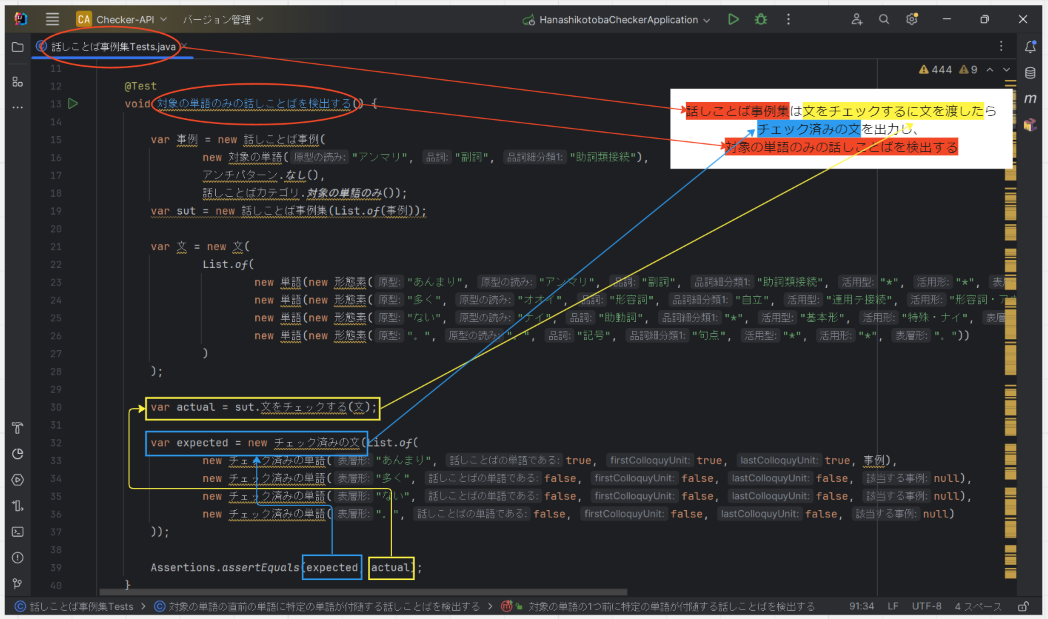
\includegraphics[width=1\linewidth]{image/testDoc.png}
\caption{テストコードの文書化の例}
\label{fig:enter-label}
\end{figure}
\section{評価結果と考察}
\subsection{責務を分けたコード}
jPeekを用いて5つの指標について算出した結果を表5.1に示す。
\begin{table}[H]
\centering
\caption{jPeekによる算出結果}
\label{ttt}
\resizebox{\textwidth}{!}{%
\begin{tabular}{ | c | c | c | c | c | c | } \hline
~&CAMC&LCOM5&MMAC&NHD&SCOM\\ \hline\hline
リファクタリング前&0.97&0.50&0.50&9.32&0.50 \\ \hline
リファクタリング後&2.81&1.06&1.24&6.62&2.42\\ \hline
\end{tabular}%
}
\end{table}
CAMCはスコアが増加した。CAMCはクラス内の型の数が増加することでスコアが増加する。クラス内の型の数が増加した要因として、リファクタリングを経てプリミティブ型が減少したことが挙げられる。このことから、リファクタリング前にあった型がメンタルモデル独自の型に置き換わったと分かる。
\\ LCOM5はスコアが増加した。LCOM5はクラス内のattributesが減少することでスコアが増加する。クラス内のattributesが減少した要因として、クラス内で用いる変数やオブジェクトが限定的になったことが挙げられる。このことから、リファクタリングを経てクラス内の責務が減少したことが考えられる。
\\ MMACはスコアが増加した。MMACはメソッドの数に対する戻り値の型の種類が減少することでスコアが増加する。メソッドの数に対する戻り値の型の種類が減少した要因として、メソッドの数自体が減少したことが挙げられる。このことから、リファクタリングを経てクラス内の責務が減少したことが考えられる。
\\ NHDはスコアが減少した。NHDは型の数が減少することでスコアが増加する。クラス内の型の数が増加した要因として、リファクタリングを経てプリミティブ型が減少したことが挙げられる。このことから、リファクタリング前にあった型がメンタルモデル独自の型に置き換わったと分かる。
\\ SCOMはスコアが増加した。SCOMは類似したメソッドが増加することでスコアが増加する。類似したメソッドが増加した要因として、リファクタリングを経てメソッドに含まれるのattributesの種類が同じになったこと、濃度が均一になったことが挙げられる。このことから、リファクタリングを経てメソッド内の責務の量が均一になったと考えられる。
\\ クラス内の責務が減少したこと、また責務の量が均一になったと考えられることから、凝集度を用いて責務を分けたコードとなっているか評価できると言える。メンタルモデルをプログラムコードに反映したことで、CAMCやNHDといった凝集度にも影響を及ぼしたことも分かる。
\subsection{共有されたメンタルモデルを反映させたコード}
シーケンス図を用いてリファクタリング前後のプログラムコードを文書化したものを以下の図5.1と図5.2に示す。
\begin{figure}[H]
\centering
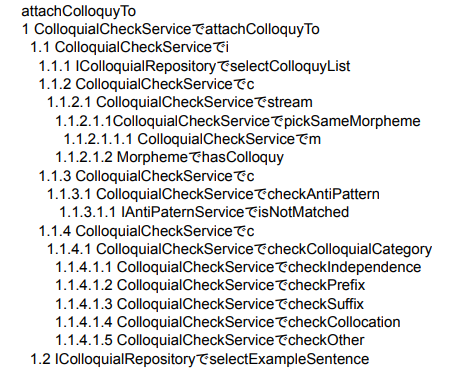
\includegraphics[width=1\linewidth]{image/modeiBe.png}
\caption{リファクタリング前のプログラムコードの文書化}
\label{fig:enter-label}
\end{figure}
\begin{figure}[H]
\centering
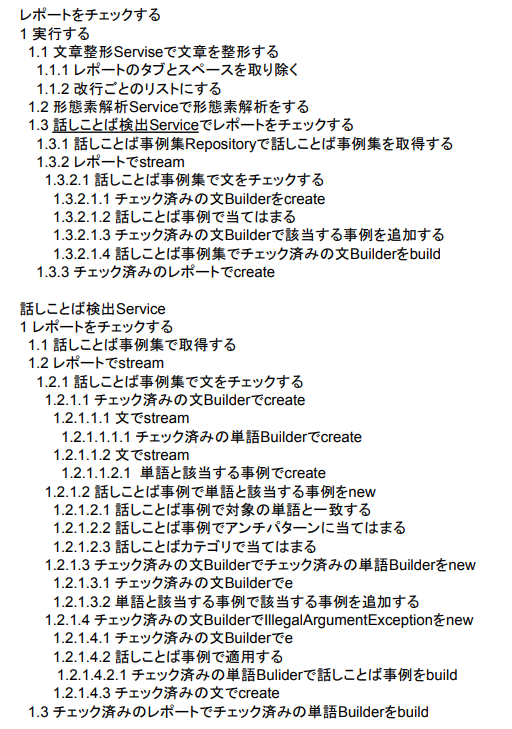
\includegraphics[width=1\linewidth]{image/modelAf.png}
\caption{リファクタリング後のプログラムコードの文書化}
\label{fig:enter-label}
\end{figure}
これらの文書を比較しリファクタリングを経て共有されたメンタルモデルを反映できているか、インタビューを行った。
\\ まず、「メンタルモデルが合っているか」について、リファクタリング後の方が山下の解釈に合っているという結果となった。そのように判断した理由として、文書の内容が日本語で記述されていることが挙げられた。「話しことば事例集は文をチェックするに文を渡したらチェック済みの文を出力する」という山下の論文には記述されていない処理の流れに関しても、山下の話しことば事例集の解釈の中にあったことが確認できた。
\\ 次に、「メンタルモデルが合っている部分はコードに直接メンタルモデルを表現できているか」について、「話しことば事例集」という山下の論文に合わせた表現を使用したことについては、分かりやすくなったという反応であった。ただし、「事例集」という表現を利用して「事例」という表現で記述した部分については文書だけでは伝わらず、口頭で説明を加えることで理解を得た。"C2Eins"などの表現をやめて、「対象の単語の一つ前に特定の単語が不随」などの山下の論文の言葉を使ったことについても、説明として分かりやすくなったという返答だった。また、streamやbuilder、iやeなどシステム開発上の入らざるを得ない言葉については理解を得られず、口頭で説明を加えた。文書化する際に用いた「で」という助詞にも正しい助詞であるのかと、疑問を抱いていた箇所があった。リファクタリング前の文書もリファクタリング後の文書もなんとなく理解できるが、リファクタリング前は英語で記述されているため、語句の理解に時間を要する結果となった。
\\ これらの結果から、ドメインモデルの構造や表現を利用したことで、共有されたメンタルモデルを部分的に反映することができたと考えられる。また、シーケンス図を基に作成した文書で開発者のメンタルモデルを共有することができることも明らかになった。ドメインエキスパートに「事例集」は伝わったが「事例」については疑問を抱いていたことから、ドメインモデルを吸い上げる際に使用するドキュメントに記載されていない言葉でプログラムコードを表現する場合には、開発者のメンタルモデルと異なる意味で捉えられる可能性があるので、ドメインエキスパートとの会話等で再定義するべきものがあると考えられる。本研究の評価では、シーケンス図のメッセージを特段選ばず、全てのメッセージを文書化したが、"stream"や"builder", "i", "e"といったシステム開発上の都合で存在しているメッセージに関しては、理解の妨げになっている様子も見られた。このことから、シーケンス図を用いてプログラムコードの文書化を行う際には、システム開発上の都合で存在しているメッセージは分かりやすい別の言葉で置き換えること、または置き換えた言葉との対応表を用意すること、または意図的に隠すこと等といった、メンタルモデルを共有しやすい文書となるよう考慮する必要がある。
\subsection{観察可能な振る舞いを確認できるコード}
テストコードを文書化したものを図5.3に示す。
\begin{figure}[H]
\centering
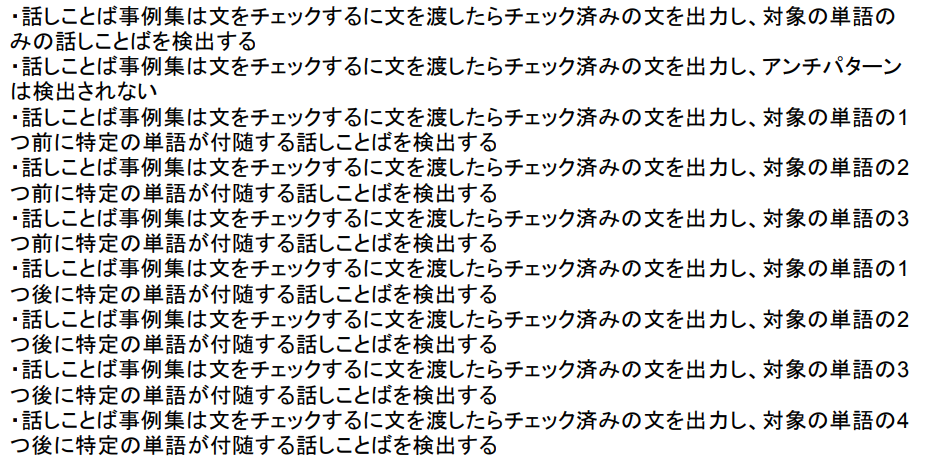
\includegraphics[width=1\linewidth]{image/hurumai.png}
\caption{テストコードの文書化}
\label{fig:enter-label}
\end{figure}
これを用いて、期待する操作と結果を確認できるかどうか、インタビューを行った。
\\ 結果としては箇条書き3つ目以降の「対象の単語の前後に特定の単語が不随する話しことば」について、期待する操作と結果として認識していなかったことが明らかになった。山下の論文では「対象の単語のみ」と「対象の単語の前に特定の単語が不随する」、「対象の単語の後に特定の単語が不随する」という言葉の記載がある。「特定の単語が付随するか」を判断する際に、「1つ前、2つ前、3つ前」や「1つ後、2つ後、3つ後、4つ後」といった特定の位置の単語を用いるものがあり、それをプログラムコードでは「対象の単語の前に特定の単語が不随する」、「対象の単語の後に特定の単語が不随する」という言葉に位置を示す数字を織り込んで表現していた。しかし、ドメインエキスパートはそれをインタビュー時に把握していなかった。
\\ 以上から、ドメインエキスパートが把握していないドメインに関する具体的な振る舞いについても、本評価で使用した文書を用いることで確認できることが明らかになった。また、箇条書き3つ目以降の振る舞いに関しては、ドメインエキスパートのメンタルモデルにはなかったことも分かる。振る舞いの確認を行うことでドメインエキスパートのメンタルモデルも確認することができたと考えられる。
\\ また、リファクタリング後にテストコードを実行したところ、全てのテストケースをクリアしたので、リファクタリング前後で振る舞いが変化していないことを確認できた。
\chapter{結論}
\section{まとめ}
本研究ではプログラムコードから要件や設計を読み取り理解することの難しさに着目し、プログラムコードの複雑さの防止効果が高いシステム開発上の要素と、それがプログラムコードに反映されているか評価する方法について検討した。
\\ 複雑化が進んだプログラムコードとなっているシステムである、「話しことばチェッカー」を研究の対象とし、複雑さの原因を分析したところ「どのような役割がどこに書かれているのか分からないコード」「開発者の独自の解釈を反映させたコード」「どのような操作でどのような結果を示すのか分からないコード」となっていることが原因であると分かった。これらを改善する方法として、ドメインエキスパートである山下の論文を用いたモデリングと、プレゼンテーション層とドメイン層にテストコードを作成することを提案し、リファクタリングでの改善を試みた。その結果、複雑さの原因が改善し、複雑さの防止効果が高いシステム開発上の要素が「責務を分けたコード」「共有されたメンタルモデルを反映させたコード」「観察可能な振る舞いを確認できるコード」であることが判明した。
\\ この3つの要素がプログラムコードに反映されているか評価する方法について、「責務を分けたコード」に関しては凝集度による評価、「共有されたメンタルモデルを反映させたコード」と「観察可能な振る舞いを確認できるコード」についてはプログラムコードやテストコードをドキュメント化したものを用いたドメインエキスパートへのインタビューにより評価を行った。それぞれの要素に関して、リファクタリング前とリファクタリング後で凝集度のスコアや、メンタルモデルや振る舞いに対するドメインエキスパートからの理解の得られやすさが変化し、これらの評価方法で3つの要素がプログラムコードに反映されているか評価できることが明らかになった。これにより、責務が分けられたコードであるか誰もが確認できる方法、メンタルモデルや観察可能な振る舞いを誰もが共有できる方法を実現できる可能性が見えたといえる。
\section{今後の課題}
 本研究では責務を分けたコードとなっているか凝集度を用いて評価することができると明らかになったが、凝集度の値がどの範囲であれば、システム開発を行う中でプログラムコードの複雑さを防止・改善することに利用できるかまでは判明していない。そこで今後の課題として、各指標についてクラスごとの評価を行うこと、別のシステムに対して同様に凝集度での評価を行い、本研究で研究対象としたシステムの結果とそれぞれのプログラムコードの責務について比較することなどで、凝集度の適切な値について検証する必要がある。
\\ メンタルモデルの共有については、本研究の結果から文書化の方法や手順について再検討しよりメンタルモデルを共有しやすい文書が作成できるようにしていくこが今後の課題として挙げられる。また、実際のシステム開発プロジェクトに本研究の評価方法を取り入れることで、メンタルモデルの共有を行うことができるか実証実験を行うことも必要である。
\\ 一般的にテストコードを作成することは難しいとされており、本研究でも観察可能な振る舞いであるかを考慮しながらのテストコード作成には多くの議論を行った。そこで、学生がテストコードを作成することをサポートできるような環境やツール、教育モデル等を提案していくことも今後の課題である。
\renewcommand{\bibname}{参考文献}
\addcontentsline{toc}{chapter}{参考文献}
\begin{thebibliography}{20}
\bibitem{haikei}「認知負荷を減らしたプログラミング学習支援に関する研究」石井 元規, 松本 慎平, 林 雄介, 平嶋 宗, 教育システム情報学会 2016年度学生研究発表会, p175-176
\bibitem{CyberZ}「良いコードとは何か」森 篤史, 2021年度 株式会社サイバーエージェント エンジニア新卒研修
\url{https://note.com/cyberz_cto/n/n26f535d6c575#HPZ6C} 2024年1月閲覧
\bibitem{kireina}「動作するきれいなプログラムを継続的に記述していくための方策について」松田 俊寛, ITJ 2015.12 第16号, p54-59
\bibitem{Domein}「ドメイン駆動設計によるシステム開発」清田 康介, 知的資産創造 2020年9月号, p116-p123
\bibitem{Yamashita}「話しことばチェッカーの開発と実証評価」山下 由美子, 長谷川 哲生, 山川 広人, 小松川 浩, 教育システム情報学会(JSiSE)2019年度 第5回研究会, p99-104
\bibitem{Tantai}「単体テストの考え方/使い方」Vladimir Khorikov, 須田 智之, 株式会社マイナビ出版, p3-10, p140-154, 2022
\bibitem{jPeek}
\end{thebibliography}

\chapter*{謝辞}
\addcontentsline{toc}{chapter}{謝辞}
\end{document}
